%\newpage
\section{Измерение резисторов}
Каждый резистор измерен четырьмя различными типами измерения в одном направлении тока. Тот же самый  резистор 
также измерен теми же самыми четырьмя типами измерения в другом направлении тока. Измерение в противоположном 
направлении используется только для того, чтобы идентифицировать резистор. Если несоответствие между обоими 
измерениями слишком большое, то это не резистор.

\subsection{Измерение резистора с резисторами 680 Ом}
Измерение неизвестного резистора Rx осуществляется двумя способами с использованием прецизионных резисторов
 \(680~\Omega\). Упрощенная схема этого измерения для испытательных выводов 1 (TP1) и 3 (TP3) показана на 
рисунках~\ref{fig:RL1mes} и~\ref{fig:RL2mes} как пример шести выбранных комбинаций испытания.

\begin{figure}[H]
\centering
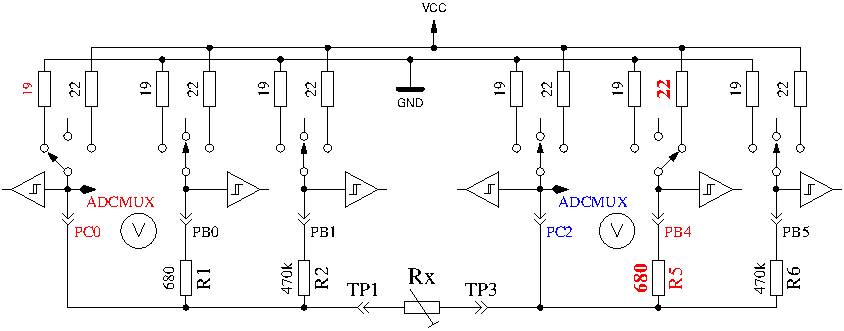
\includegraphics[width=.8\textwidth]{../FIG/ResistormessL1.pdf}
\caption{Измерение Типа 1 с резистором \(680~\Omega\) }
\label{fig:RL1mes}
\end{figure}

\begin{figure}[H]
 \centering
 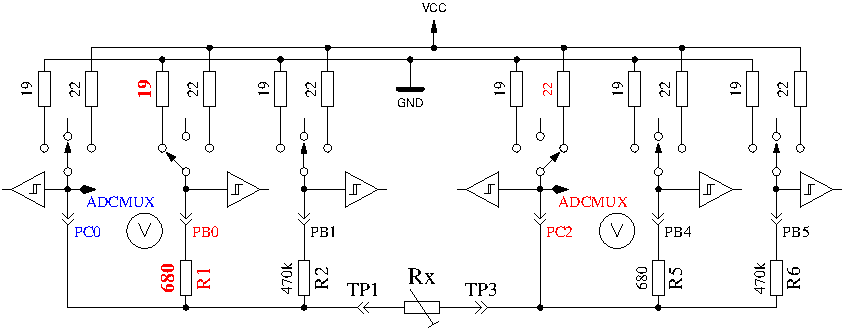
\includegraphics[width=.8\textwidth]{../FIG/ResistormessL2.pdf}
 \caption{Измерение Типа 2 с резистором \(680~\Omega\) }
\label{fig:RL2mes}
\end{figure}


С левой стороны расположен испытательный вывод 1, с правой стороны - испытательный вывод 3. В обеих диаграммах 
Вы видите, что вывод 3 (правая сторона) соединён с VCC, вывод 1 (левая сторона) соединен с GND. Направление тока, 
текущего через резистор Rx является одинаковым. Значения  портов, переключенных на выход, показаны красным цветом, 
значения портов, используемых в качестве входа, отображаются синим цветом, бездействующие порты - черные. В обоих 
показанных типах измерения ток должен быть одинаковым, потому что суммарная величина резисторов между VCC и GND 
идентична (если измерительные резисторы одинаковые – в идеальном случае). Обычно измеренное напряжение не 
одинаковое, потому что меняются подключенные резисторы. 
Символ V на диаграмме отмечает порты, используемые для измерения напряжения. В обеих конфигурациях величина 
резистора Rx может быть вычислена по известной величине резистора и измеренному напряжению, если отношение 
резистора Rx к \(680~\Omega\) не слишком велико. Теоретическое отклонение напряжения показано на 
рисунке~\ref{fig:RLvtot}, где величина резистора показана в логарифмическом масштабе.
\begin{figure}[H]
\centering
\includegraphics[width=.93\textwidth]{../GNU/RLvtotRU.pdf}
\caption{Напряжение при измерениях Типа 1 и Типа 2 с резистором \(680~\Omega\) }
\label{fig:RLvtot}
\end{figure}
График  измерения Типа 1 показан  на  рисунке~\ref{fig:RLvlow} с измененным масштабом изображения для малых 
значений резисторов. Здесь видно, что для получения точного измерения величины резистора ниже \(2~\Omega\)
необходимо лучшее разрешение АЦП, чем стандартное разрешение \(4,9~mV\) с \(5~V\) ИОН.  Есть только 3 отсчета 
АЦП от \(0~\Omega\) до \(2~\Omega\).
Опция AUTO\_SCALE\_ADC, переключающая диапазон АЦП, может помочь в этом случае. Тот же самый участок с измененным 
масштабом изображения диапазона измерения Типа 2 показан на рисунке~\ref{fig:RLvhigh}.
К сожалению, мы не можем использовать высокое разрешение АЦП для измерения типа~2 в этом диапазоне, потому что 
напряжение слишком высоко, а у применённых ATmega нет дифференциального входа АЦП. Измерения с 
резисторами \(680~\Omega\) проводятся для получения результата измерений до \(20~k\Omega\)
(измеренное напряжение типа~2 будет ниже \(169~mV\)).

Для более высоких значений измеряемого резистора измерения  проводятся с резисторами \(470~k\Omega\). Если все 
тесты свидетельствуют о том, что это не другой тип элемента, то полученная величина обоих измерений берется в 
качестве величины сопротивления резистора для отображения на дисплее. Если выбрана опция AUTO\_SCALE\_ADC, и 
одно из напряжений обоих типов измерения ниже \(0,98~V\), взвешенное среднее значение вычисляют с коэффициентом 4 
для этой величины. Другая взвешенная величина имеет коэффициент 1. Это сделано для того, чтобы предпочесть 
коэффициент 4 для лучшего разрешения этого измерения. Коэффициент 4 взят только для микроконтроллеров ATmega168 
и ATmega328, для ATmega8 в качестве весового коэффициента взято 2, если напряжение ниже \(0.98~V\), потому что опорное 
напряжение для АЦП ATmega8 \(2,54~V\) вместо \(1,1~V\) для ATmega168 и ATmega328. Для ATmega168 и ATmega328 измерение 
напряжения на резисторах будет задержано, пока не обнаружатся большие изменения или закончится лимит времени. 
При использовании этого метода большие конденсаторы более не определяются, как резисторы, по ошибке, и 
сопротивление постоянному току больших катушек индуктивности будет измерено правильно.


\begin{figure}[H]
  \begin{subfigure}[b]{.5\textwidth}
    \centering
    \includegraphics[width=1.\textwidth]{../GNU/RLvlowRU.pdf}
    \caption{Измерение Типа 1}
    \label{fig:RLvlow}
  \end{subfigure}
  ~
  \begin{subfigure}[b]{.5\textwidth}
    \centering
    \includegraphics[width=1.\textwidth]{../GNU/RLvhighRU.pdf}
    \caption{Измерение Типа 2}
    \label{fig:RLvhigh}
  \end{subfigure}
  \caption{Теоретическое напряжение от \(0~\Omega\) до \(10~\Omega\)}
\end{figure}


\subsection{Измерение резистора с резисторами 470 кОм}
Следующие рисунки~\ref{fig:RH1mes} и \ref{fig:RH2mes} показывают ту же самую процедуру измерения с прецизионными 
резисторами \(470~k\Omega\). Поскольку \(470~k\Omega\) очень большие относительно величины резистора 
порта \(19~\Omega\) или \(22~\Omega\), величины резисторов портов не учитываются для вычисления величины резистора Rx.

Для обоих Типов измерения с резисторами \(470~k\Omega\) измеряется только одно напряжение, потому что ток настолько 
низок, что никакое различие напряжения во внутренних резисторах порта ATmega не может быть измерено (как и 
ожидалось). Теоретическое отклонение напряжения показано на рисунке~\ref{fig:RHv} где величина резистора показана 
в логарифмическом масштабе. Теоретическое отклонение в этой диаграмме заканчивается на \(100~M\Omega\), но 
фактическое значение для Тестера ограничено \(60~M\Omega\), иначе Тестер определяет, что резистор не подключен. 
Взвешенное среднее число обоих Типов измерения взято в качестве результата с теми же самыми коэффициентами, 
описанными для измерений с резисторами \(680~\Omega\).
Для всех микроконтроллеров ATmega я определил, что взвешенные результаты с резисторами \(470~k\Omega\) более точны, 
если будет добавлено постоянное смещение \(350~\Omega\).
Этот смещение может быть подобрано определением величины RH\_OFFSET в файле config.h

\begin{figure}[H]
\centering
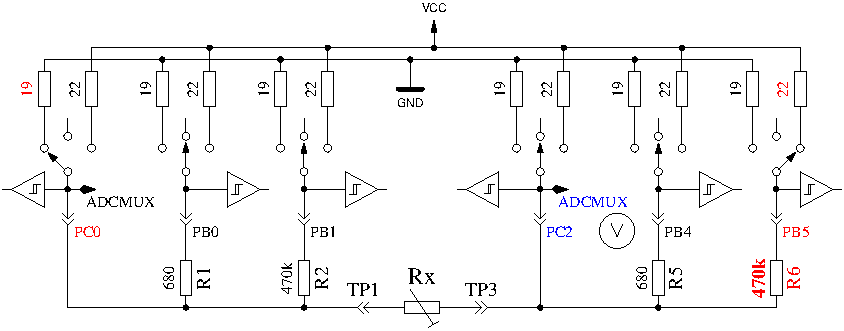
\includegraphics[width=.8\textwidth]{../FIG/ResistormessH1.pdf}
\caption{Измерение Типа 3 с резистором \(470~k\Omega\) }
\label{fig:RH1mes}
\end{figure}

\begin{figure}[H]
 \centering
 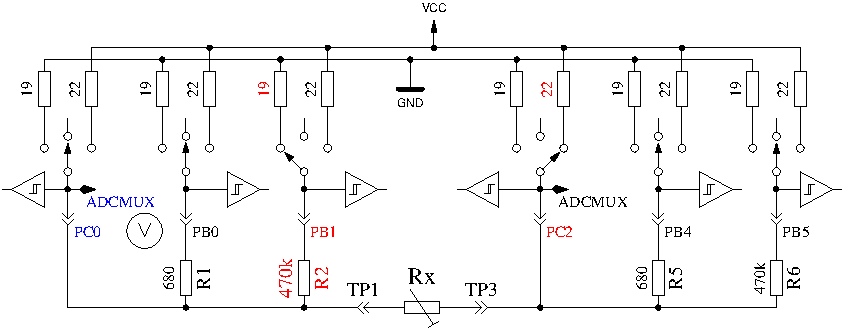
\includegraphics[width=.8\textwidth]{../FIG/ResistormessH2.pdf}
 \caption{Измерение Типа 4 с резистором \(470~k\Omega\) }
\label{fig:RH2mes}
\end{figure}

\begin{figure}[H]
\centering
\includegraphics[width=.93\textwidth]{../GNU/RHvRU.pdf}
\caption{Напряжение при измерениях Типа 3 и Типа 4 с резистором \(470~k\Omega\) }
\label{fig:RHv}
\end{figure}

\subsection{Результаты измерений резистора}
Рисунок~\ref{fig:mega8res} показывает относительную погрешность измерений резистора тремя ATmega8 . Дополнительно 
приведены результаты с оригинальным программным обеспечением от Markus~F. (\inquotes{Mega8orig}) с одним ATmega8. На 
рисунках~\ref{fig:mega8Ares} и \ref{fig:mega8Lres} показаны результаты измерений с ATmega8A и ATmega8L. 
Рисунок~\ref{fig:mega168res} показывает те же самые измерения с ATmega168 (Mega168 - результаты без опции 
AUTOSCALE\_ADC, Mega168as - те же самые измерения с опцией AUTOSCALE\_ADC). Применение ATmega168 дает возможность 
измерения резисторов в диапазоне от \(20~\Omega\) до \(20~M\Omega\) с точностью \(\pm1\%\).
Для измерений ниже \(100~\Omega\) Вы должны иметь в виду, что любые измерительные провода также имеют сопротивление. 
Лучше подсоединить резистор непосредственно к контактам терминала. Если это невозможно, вычтите величину 
сопротивления, измеренную с закороченными щупами. Например, если резистор маркирован \(30~\Omega\) и Тестер 
показывает величину \(30,6~\Omega\),
а у закороченных щупов замерена величина \(0,5~\Omega\), то измеренная величина резистора составит \(30,1~\Omega\).
Для сопротивлений ниже \(10~\Omega\) один отсчет  разрешения даёт ошибку больше, чем 1\%!

\begin{figure}[H]
\centering
\includegraphics[width=.93\textwidth]{../GNU/Mega8resRU.pdf}
\caption{Относительная погрешность измерений резисторов на ATmega8 }
\label{fig:mega8res}
\end{figure}

\begin{figure}[H]
  \begin{subfigure}[b]{.5\textwidth}
    \centering
    \includegraphics[width=1.\textwidth]{../GNU/Mega8AresRU.pdf}
    \caption{ATmega8A}
    \label{fig:mega8Ares}
  \end{subfigure}
  ~
  \begin{subfigure}[b]{.5\textwidth}
    \centering
    \includegraphics[width=1.\textwidth]{../GNU/Mega8LresRU.pdf}
    \caption{ATmega8L}
    \label{fig:mega8Lres}
  \end{subfigure}
\caption{Относительная погрешность измерений резисторов}
\end{figure}


\begin{figure}[H]
\centering
\includegraphics[width=.93\textwidth]{../GNU/Mega168resRU.pdf}
\caption{Относительная погрешность измерений резисторов на ATmega168 }
\label{fig:mega168res}
\end{figure}

Рисунок~\ref{fig:m168res_all} показывает погрешность измерения для трех микроконтроллеров ATmega168 перед 
калибровкой - точками, после калибровки - линией. Аналогичная погрешность измерения для трех ATmega168A показана 
на рисунке~\ref{fig:m168ares_all} а погрешность измерения для трех ATmega168P показана на 
рисунке~\ref{fig:m168pres_all} .
Погрешность измерения для трех ATmega328 показана на рисунках~\ref{fig:m328res_all} и \ref{fig:m328pres_all}.
После автокалибровки относительная погрешность измерения резисторов в диапазоне от \(10~\Omega~-~20~M\Omega\) 
обычно находится в пределах \(\pm1~\%\). Только одно измерение резистора \(22~k\Omega\) с ATmega328P-13 показывает 
более высокую погрешность. Перед калибровкой погрешность некоторых микроконтроллеров составляла \(\pm~3\%\).
Это было скорректировано переключением опоры АЦП опцией AUTOSCALE\_ADC. Прямое сравнение напряжения на конденсаторе 
ниже \(1~V\), однократно измеренного с опорой VCC, и другое однократное измерение с внутренней опорой, может подстроить 
эту погрешность. Измерение напряжения производится тем же самым каналом мультиплексора, а внутренняя опора связана 
с выводом AREF ATmega. К сожалению, прямое измерение опоры со своим каналом мультиплексора приводит к смещению, 
которое  может быть вручную подстроено опцией  REF\_R\_KORR или автоматически опцией самопроверки AUTO\_CAL. 
Значение REF\_R\_KORR является дополнительным смещением к автоматически определённому значению с опцией AUTO\_CAL!

\begin{figure}[H]
  \begin{subfigure}[b]{.5\textwidth}
    \centering
    \includegraphics[width=1.\textwidth]{../GNU/m168res_allRU.pdf}
    \caption{ATmega168}
    \label{fig:m168res_all}
  \end{subfigure}
  ~
  \begin{subfigure}[b]{.5\textwidth}
    \centering
    \includegraphics[width=1.\textwidth]{../GNU/m168ares_allRU.pdf}
    \caption{ATmega168A}
    \label{fig:m168ares_all}
  \end{subfigure}
\caption{Относительная погрешность измерений резисторов}
\end{figure}

\begin{figure}[H]
\centering
\includegraphics[width=.93\textwidth]{../GNU/m168pres_allRU.pdf}
\caption{Относительная погрешность измерений резисторов на ATmega168P }
\label{fig:m168pres_all}
\end{figure}

\begin{figure}[H]
  \begin{subfigure}[b]{.5\textwidth}
    \centering
    \includegraphics[width=1.\textwidth]{../GNU/m328res_allRU.pdf}
    \caption{ATmega328}
    \label{fig:m328res_all}
  \end{subfigure}
  ~
  \begin{subfigure}[b]{.5\textwidth}
    \centering
    \includegraphics[width=1.\textwidth]{../GNU/m328pres_allRU.pdf}
    \caption{ATmega328P}
    \label{fig:m328pres_all}
  \end{subfigure}
\caption{Относительная погрешность измерений резисторов}
\end{figure}

